%!TEX root = ../report.tex
\newpage
\section{Risk assessment}
The system is confronted by several risks which are determined and mitigated in this section.
Taking those risks into account allows to avoid them or at least reduce their impact. 
The risk management involves the identification of the risks, their probability and potential impact or consequences.

The tables below explain the meaning of the definition for probability and consequence.
\begin{figure}[h]
\centering
\begin{tabular}{|c|c|}
\hline \textbf{Probability} & \textbf{Likelihood of occurrence} \\ 
\hline High & 0.65 - 1.00 \\ 
\hline Medium & 0.35 - 0.65 \\ 
\hline Low & 0.00 - 0.35 \\ 
\hline
\end{tabular} 
\label{table:risk-probability}
\end{figure}

\begin{figure}[h]
\centering
\begin{tabular}{|l|p{15.5cm}|}
\hline \textbf{Severity} & \textbf{Explanation} \\ 
\hline Severe & A risk that can lead to loss of live or casualties. \\ 
\hline Significant & A risk that can lead to damages, can delay the project more than 3 months or causes one of the high-level requirements not to be fulfilled. \\ 
\hline Moderate & A risk that can lead to one of the high-level requirements not to be fulfilled to an acceptable level. \\ 
\hline Minor & A risk that can lead to one of the high-level requirements not being fully fulfilled, but still fulfilled in an acceptable level. \\
\hline
\end{tabular} 
\label{table:risk-severity}
\end{figure}

%Risk impact assesment and Prioritization
% Probability of Occurrence ( In the appendice is the table to which show how to evaluate a risk and the severity of consequences 
%\textit{http://www.mitre.org/publications/systems-engineering-guide/acquisition-systems-engineering/risk-management/risk-impact-assessment-and-prioritization} \\ % COSTS
%Timeframe is classified in : Long , Medium , Short , Imminent \\
%Consequences are classified in : Low, Moderate , High , Severe


%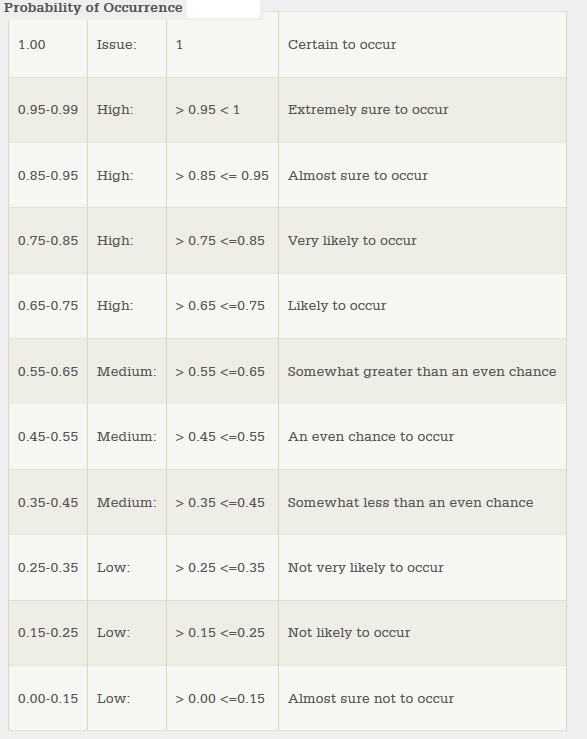
\includegraphics[scale=0.5]{3-requirements/Images/RISKSOCCURENCE.jpg} % maybe in the appendice ?
\subsection{Technical}

\risk{T}
{The system does not detect a flood}
{Low}
{Severe. There can be a loss of human lives and damages, loss of trust in the system by end-users.}
{Make sure the number of sensors is sufficient and that they are in good state (as low failure rate as possible, when necessary repair or replace them). Perform regular checks of the sensors.}
{Make changes in the algorithm for the flood detection, improve the sensors used or add more sensors.}

\risk{T}
{The system sends warnings of a non-existing flood (false positive)} % WHEN THERE IS A FLOOD YOU KNOW IT
{Low}
{Significant. People can become more negligent to future messages and unneeded social disturbance can be caused.}
{UAVs watching the area where the supposed flood is to confirm.}
{Send a message as soon as the mistake is detected to tell the population/emergency center it was a false alert. }

\risk{T}
{The system cannot send messages to the necessary people because the communication platform is also destroyed by the flood}
{Medium}
{Severe. If the warning is not send, the area might not be evacuated timely. Potential loss of human lives, casualties and damages to property. }
{}
{Send the warning to the government using a different medium.}
	
%\risk{T}
%{The system sends incorrect information}
%{Low}
%{Severe. Loss of money and maybe lives.}
%{Operator checking the validity of the information sent by the system.
%	Good collaboration with the insurance companies.}
%{  }
% WM: Risk and severity depend highly on what kind of information is send incorrectly.

\risk{T}
{Hacker gets access to the system}
{Low}
{Severe. The hacker may sent incorrect information deliberately during the flood. This can cause unneeded evacuation, but in the case of a flood also loss of human lives. The system is not reliable anymore.}
{Change password and hash codes every three months. Hire specialists in the security field to audit the security system on a regular basis (penetration testing).}
{Update the security system / change it. Find a new algorithm for the creation of password and hash codes.}



\subsection{Business}

\risk{B}
{Wrong estimation of the budget}
{Medium}
{Significant. The final product does not have the features expected.}
{The team needs an accountant or at least someone taking care of the follow-up of the money. Make sure there are regular evaluations to keep track of the money flow.}
{Remove some requirements or features of the product, or change the hardware components used.}

\risk{B}
{The money invested in the fabrication and achievement of the product/system is not covered by the sales (shortfall/deficit)}
{Medium}
{Moderate. Stopping the sale}
{The team needs an accountant or at least someone taking care of the follow-up of the money.}
{Adding more features to the product in order to make it more competitive in the market.}

%\risk{B}
%{Competitors lowering their prices}
%{Medium}
%{Moderate. Loss of money.}
%{  }
%{  }
% WM: I think this one is too generic
	
\risk{B}
{Sensor becomes unavailable (is not sold anymore)}
{Medium}
{Moderate. Sensors will fail and need replacing over time, if new sensors are not available anymore, this becomes impossible.}
{ Choose a sensor that is not too old and is expected to be available for at least the next 5 years. }
{ Use a different sensor and modify the system so it can operate with this sensor. }	

	%\textbf{ B-RISK4 The sensors company become bankrupt or at least stops its sales.} \\
	%\textit{Probability of Occurence}: Low \\
	%\textit{Consequences}: High.\\
	%\textit{Prevention} Our system use sensors from different companies \\
	%\textit{Decision}: Find another company selling sensors and make sure of its reliability. \\


\subsection{Schedule}
\risk{S}
{The project is not finished at the deadline}
{Low}
{Significant. Pressure for all the team members, loss of credibility regarding the customers, selling a product with less features than expected.}
{ Meeting for the team members every week to keep track of the timing and take decisions according to the deadline. }
{ Remove some requirements or features in order to finish the project as soon as possible. }